

\tikzset{every picture/.style={line width=0.75pt}} %set default line width to 0.75pt        

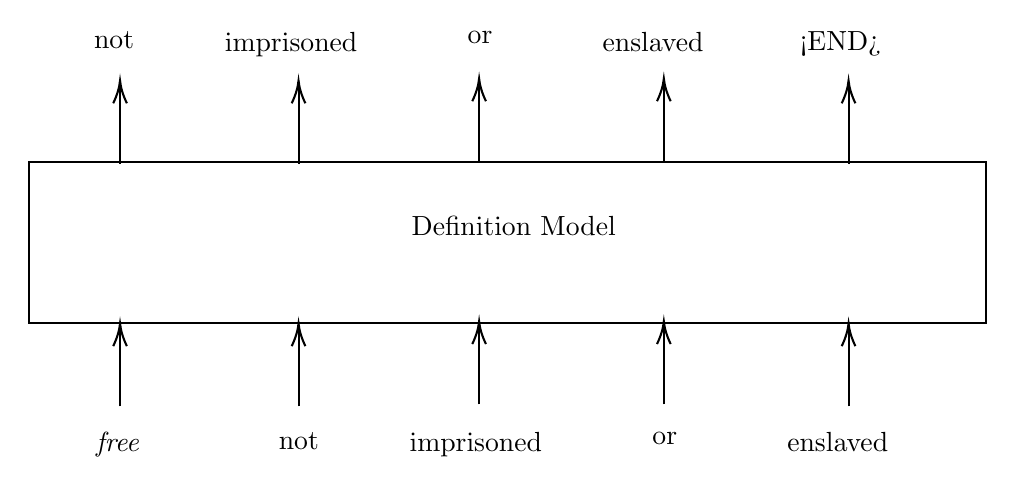
\begin{tikzpicture}[x=0.75pt,y=0.75pt,yscale=-1,xscale=1]
    %uncomment if require: \path (0,300); %set diagram left start at 0, and has height of 300

    %Shape: Rectangle [id:dp6814608191560567] 
    \draw   (106,135.18) -- (567.01,135.18) -- (567.01,213) -- (106,213) -- cycle ;
    %Straight Lines [id:da8412827668688772] 
    \draw    (150,253) -- (150,215) ;
    \draw [shift={(150,213)}, rotate = 90] [color={rgb, 255:red, 0; green, 0; blue, 0 }  ][line width=0.75]    (10.93,-3.29) .. controls (6.95,-1.4) and (3.31,-0.3) .. (0,0) .. controls (3.31,0.3) and (6.95,1.4) .. (10.93,3.29)   ;
    %Straight Lines [id:da5692318832889067] 
    \draw    (236,253) -- (236,215) ;
    \draw [shift={(236,213)}, rotate = 90] [color={rgb, 255:red, 0; green, 0; blue, 0 }  ][line width=0.75]    (10.93,-3.29) .. controls (6.95,-1.4) and (3.31,-0.3) .. (0,0) .. controls (3.31,0.3) and (6.95,1.4) .. (10.93,3.29)   ;
    %Straight Lines [id:da9259697442326651] 
    \draw    (323,252) -- (323,214) ;
    \draw [shift={(323,212)}, rotate = 90] [color={rgb, 255:red, 0; green, 0; blue, 0 }  ][line width=0.75]    (10.93,-3.29) .. controls (6.95,-1.4) and (3.31,-0.3) .. (0,0) .. controls (3.31,0.3) and (6.95,1.4) .. (10.93,3.29)   ;
    %Straight Lines [id:da32056643776074534] 
    \draw    (412,252) -- (412,214) ;
    \draw [shift={(412,212)}, rotate = 90] [color={rgb, 255:red, 0; green, 0; blue, 0 }  ][line width=0.75]    (10.93,-3.29) .. controls (6.95,-1.4) and (3.31,-0.3) .. (0,0) .. controls (3.31,0.3) and (6.95,1.4) .. (10.93,3.29)   ;
    %Straight Lines [id:da8034615427684437] 
    \draw    (501,253) -- (501,215) ;
    \draw [shift={(501,213)}, rotate = 90] [color={rgb, 255:red, 0; green, 0; blue, 0 }  ][line width=0.75]    (10.93,-3.29) .. controls (6.95,-1.4) and (3.31,-0.3) .. (0,0) .. controls (3.31,0.3) and (6.95,1.4) .. (10.93,3.29)   ;
    %Straight Lines [id:da883786696743114] 
    \draw    (150,136) -- (150,98) ;
    \draw [shift={(150,96)}, rotate = 90] [color={rgb, 255:red, 0; green, 0; blue, 0 }  ][line width=0.75]    (10.93,-3.29) .. controls (6.95,-1.4) and (3.31,-0.3) .. (0,0) .. controls (3.31,0.3) and (6.95,1.4) .. (10.93,3.29)   ;
    %Straight Lines [id:da6001638094548338] 
    \draw    (236,136) -- (236,98) ;
    \draw [shift={(236,96)}, rotate = 90] [color={rgb, 255:red, 0; green, 0; blue, 0 }  ][line width=0.75]    (10.93,-3.29) .. controls (6.95,-1.4) and (3.31,-0.3) .. (0,0) .. controls (3.31,0.3) and (6.95,1.4) .. (10.93,3.29)   ;
    %Straight Lines [id:da6543230843272436] 
    \draw    (323,135) -- (323,97) ;
    \draw [shift={(323,95)}, rotate = 90] [color={rgb, 255:red, 0; green, 0; blue, 0 }  ][line width=0.75]    (10.93,-3.29) .. controls (6.95,-1.4) and (3.31,-0.3) .. (0,0) .. controls (3.31,0.3) and (6.95,1.4) .. (10.93,3.29)   ;
    %Straight Lines [id:da6603420484640341] 
    \draw    (412,135) -- (412,97) ;
    \draw [shift={(412,95)}, rotate = 90] [color={rgb, 255:red, 0; green, 0; blue, 0 }  ][line width=0.75]    (10.93,-3.29) .. controls (6.95,-1.4) and (3.31,-0.3) .. (0,0) .. controls (3.31,0.3) and (6.95,1.4) .. (10.93,3.29)   ;
    %Straight Lines [id:da6434927779308499] 
    \draw    (501,136) -- (501,98) ;
    \draw [shift={(501,96)}, rotate = 90] [color={rgb, 255:red, 0; green, 0; blue, 0 }  ][line width=0.75]    (10.93,-3.29) .. controls (6.95,-1.4) and (3.31,-0.3) .. (0,0) .. controls (3.31,0.3) and (6.95,1.4) .. (10.93,3.29)   ;

    % Text Node
    \draw (289,160) node [anchor=north west][inner sep=0.75pt]   [align=left] {Definition Model};
    % Text Node
    \draw (137,264) node [anchor=north west][inner sep=0.75pt]   [align=left] {\textit{free}};
    % Text Node
    \draw (136,71) node [anchor=north west][inner sep=0.75pt]   [align=left] {not};
    % Text Node
    \draw (199,71) node [anchor=north west][inner sep=0.75pt]   [align=left] {imprisoned};
    % Text Node
    \draw (316,71) node [anchor=north west][inner sep=0.75pt]   [align=left] {or};
    % Text Node
    \draw (381,71) node [anchor=north west][inner sep=0.75pt]   [align=left] {enslaved};
    % Text Node
    \draw (476,71) node [anchor=north west][inner sep=0.75pt]   [align=left] {<END>};
    % Text Node
    \draw (225,264) node [anchor=north west][inner sep=0.75pt]   [align=left] {not};
    % Text Node
    \draw (288,264) node [anchor=north west][inner sep=0.75pt]   [align=left] {imprisoned};
    % Text Node
    \draw (405,264) node [anchor=north west][inner sep=0.75pt]   [align=left] {or};
    % Text Node
    \draw (470,264) node [anchor=north west][inner sep=0.75pt]   [align=left] {enslaved};


\end{tikzpicture}
